% Generated by ArticleSignalDiagrams. Opaque vector fills only.
\documentclass[10pt,tikz,border=5pt]{standalone}
\usepackage{lmodern}
\usetikzlibrary{fit}
\begin{document}
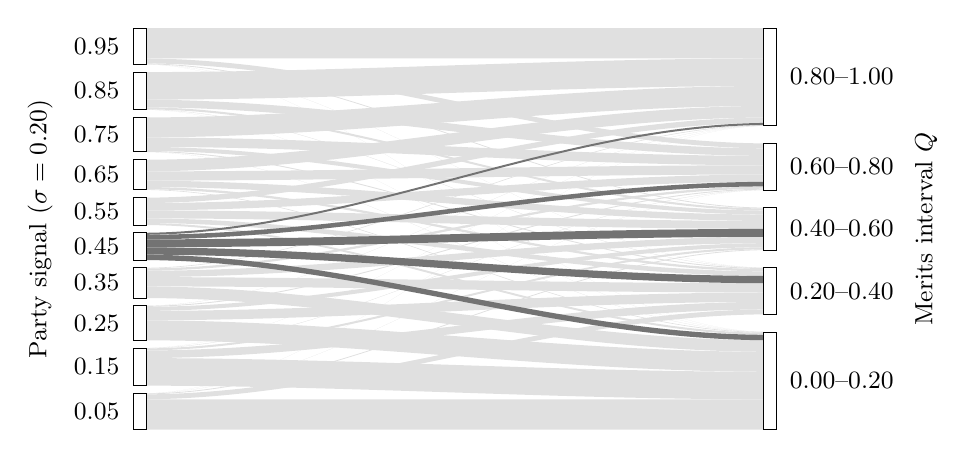
\begin{tikzpicture}[x=1cm,y=1cm,font=\small]\path[fill=black!12,draw=none] (3.3,-5.1) .. controls (6,-5.1) and (8.6,-5.1) .. (11.3,-5.1) -- (11.3,-4.714678) .. controls (8.6,-4.714678) and (6,-4.714678) .. (3.3,-4.714678) -- cycle;
\path[fill=black!12,draw=none] (3.3,-4.714678) .. controls (6,-4.714678) and (8.6,-3.635298) .. (11.3,-3.635298) -- (11.3,-3.573133) .. controls (8.6,-3.573133) and (6,-4.652514) .. (3.3,-4.652514) -- cycle;
\path[fill=black!12,draw=none] (3.3,-4.652514) .. controls (6,-4.652514) and (8.6,-2.819196) .. (11.3,-2.819196) -- (11.3,-2.808679) .. controls (8.6,-2.808679) and (6,-4.641997) .. (3.3,-4.641997) -- cycle;
\path[fill=black!12,draw=none] (3.3,-4.641997) .. controls (6,-4.641997) and (8.6,-2.055804) .. (11.3,-2.055804) -- (11.3,-2.054868) .. controls (8.6,-2.054868) and (6,-4.641061) .. (3.3,-4.641061) -- cycle;
\path[fill=black!12,draw=none] (3.3,-4.641061) .. controls (6,-4.641061) and (8.6,-1.239702) .. (11.3,-1.239702) -- (11.3,-1.239649) .. controls (8.6,-1.239649) and (6,-4.641007) .. (3.3,-4.641007) -- cycle;
\path[fill=black!12,draw=none] (3.3,-4.541007) .. controls (6,-4.541007) and (8.6,-4.714678) .. (11.3,-4.714678) -- (11.3,-4.36497) .. controls (8.6,-4.36497) and (6,-4.191299) .. (3.3,-4.191299) -- cycle;
\path[fill=black!12,draw=none] (3.3,-4.191299) .. controls (6,-4.191299) and (8.6,-3.573133) .. (11.3,-3.573133) -- (11.3,-3.476793) .. controls (8.6,-3.476793) and (6,-4.094958) .. (3.3,-4.094958) -- cycle;
\path[fill=black!12,draw=none] (3.3,-4.094958) .. controls (6,-4.094958) and (8.6,-2.808679) .. (11.3,-2.808679) -- (11.3,-2.782654) .. controls (8.6,-2.782654) and (6,-4.068934) .. (3.3,-4.068934) -- cycle;
\path[fill=black!12,draw=none] (3.3,-4.068934) .. controls (6,-4.068934) and (8.6,-2.054868) .. (11.3,-2.054868) -- (11.3,-2.051164) .. controls (8.6,-2.051164) and (6,-4.06523) .. (3.3,-4.06523) -- cycle;
\path[fill=black!12,draw=none] (3.3,-4.06523) .. controls (6,-4.06523) and (8.6,-1.239649) .. (11.3,-1.239649) -- (11.3,-1.239299) .. controls (8.6,-1.239299) and (6,-4.06488) .. (3.3,-4.06488) -- cycle;
\path[fill=black!12,draw=none] (3.3,-3.96488) .. controls (6,-3.96488) and (8.6,-4.36497) .. (11.3,-4.36497) -- (11.3,-4.111376) .. controls (8.6,-4.111376) and (6,-3.711285) .. (3.3,-3.711285) -- cycle;
\path[fill=black!12,draw=none] (3.3,-3.711285) .. controls (6,-3.711285) and (8.6,-3.476793) .. (11.3,-3.476793) -- (11.3,-3.35772) .. controls (8.6,-3.35772) and (6,-3.592213) .. (3.3,-3.592213) -- cycle;
\path[fill=black!12,draw=none] (3.3,-3.592213) .. controls (6,-3.592213) and (8.6,-2.782654) .. (11.3,-2.782654) -- (11.3,-2.731385) .. controls (8.6,-2.731385) and (6,-3.540944) .. (3.3,-3.540944) -- cycle;
\path[fill=black!12,draw=none] (3.3,-3.540944) .. controls (6,-3.540944) and (8.6,-2.051164) .. (11.3,-2.051164) -- (11.3,-2.039515) .. controls (8.6,-2.039515) and (6,-3.529295) .. (3.3,-3.529295) -- cycle;
\path[fill=black!12,draw=none] (3.3,-3.529295) .. controls (6,-3.529295) and (8.6,-1.239299) .. (11.3,-1.239299) -- (11.3,-1.23747) .. controls (8.6,-1.23747) and (6,-3.527466) .. (3.3,-3.527466) -- cycle;
\path[fill=black!12,draw=none] (3.3,-3.427466) .. controls (6,-3.427466) and (8.6,-4.111376) .. (11.3,-4.111376) -- (11.3,-3.964179) .. controls (8.6,-3.964179) and (6,-3.28027) .. (3.3,-3.28027) -- cycle;
\path[fill=black!12,draw=none] (3.3,-3.28027) .. controls (6,-3.28027) and (8.6,-3.35772) .. (11.3,-3.35772) -- (11.3,-3.240267) .. controls (8.6,-3.240267) and (6,-3.162817) .. (3.3,-3.162817) -- cycle;
\path[fill=black!12,draw=none] (3.3,-3.162817) .. controls (6,-3.162817) and (8.6,-2.731385) .. (11.3,-2.731385) -- (11.3,-2.650872) .. controls (8.6,-2.650872) and (6,-3.082304) .. (3.3,-3.082304) -- cycle;
\path[fill=black!12,draw=none] (3.3,-3.082304) .. controls (6,-3.082304) and (8.6,-2.039515) .. (11.3,-2.039515) -- (11.3,-2.010363) .. controls (8.6,-2.010363) and (6,-3.053152) .. (3.3,-3.053152) -- cycle;
\path[fill=black!12,draw=none] (3.3,-3.053152) .. controls (6,-3.053152) and (8.6,-1.23747) .. (11.3,-1.23747) -- (11.3,-1.229833) .. controls (8.6,-1.229833) and (6,-3.045515) .. (3.3,-3.045515) -- cycle;
\path[fill=black!12,draw=none] (3.3,-2.5) .. controls (6,-2.5) and (8.6,-3.895707) .. (11.3,-3.895707) -- (11.3,-3.870167) .. controls (8.6,-3.870167) and (6,-2.47446) .. (3.3,-2.47446) -- cycle;
\path[fill=black!12,draw=none] (3.3,-2.47446) .. controls (6,-2.47446) and (8.6,-3.147775) .. (11.3,-3.147775) -- (11.3,-3.089637) .. controls (8.6,-3.089637) and (6,-2.416321) .. (3.3,-2.416321) -- cycle;
\path[fill=black!12,draw=none] (3.3,-2.416321) .. controls (6,-2.416321) and (8.6,-2.55) .. (11.3,-2.55) -- (11.3,-2.449128) .. controls (8.6,-2.449128) and (6,-2.31545) .. (3.3,-2.31545) -- cycle;
\path[fill=black!12,draw=none] (3.3,-2.31545) .. controls (6,-2.31545) and (8.6,-1.952225) .. (11.3,-1.952225) -- (11.3,-1.859733) .. controls (8.6,-1.859733) and (6,-2.222957) .. (3.3,-2.222957) -- cycle;
\path[fill=black!12,draw=none] (3.3,-2.222957) .. controls (6,-2.222957) and (8.6,-1.204293) .. (11.3,-1.204293) -- (11.3,-1.135821) .. controls (8.6,-1.135821) and (6,-2.154485) .. (3.3,-2.154485) -- cycle;
\path[fill=black!12,draw=none] (3.3,-2.054485) .. controls (6,-2.054485) and (8.6,-3.870167) .. (11.3,-3.870167) -- (11.3,-3.86253) .. controls (8.6,-3.86253) and (6,-2.046848) .. (3.3,-2.046848) -- cycle;
\path[fill=black!12,draw=none] (3.3,-2.046848) .. controls (6,-2.046848) and (8.6,-3.089637) .. (11.3,-3.089637) -- (11.3,-3.060485) .. controls (8.6,-3.060485) and (6,-2.017696) .. (3.3,-2.017696) -- cycle;
\path[fill=black!12,draw=none] (3.3,-2.017696) .. controls (6,-2.017696) and (8.6,-2.449128) .. (11.3,-2.449128) -- (11.3,-2.368615) .. controls (8.6,-2.368615) and (6,-1.937183) .. (3.3,-1.937183) -- cycle;
\path[fill=black!12,draw=none] (3.3,-1.937183) .. controls (6,-1.937183) and (8.6,-1.859733) .. (11.3,-1.859733) -- (11.3,-1.74228) .. controls (8.6,-1.74228) and (6,-1.81973) .. (3.3,-1.81973) -- cycle;
\path[fill=black!12,draw=none] (3.3,-1.81973) .. controls (6,-1.81973) and (8.6,-1.135821) .. (11.3,-1.135821) -- (11.3,-0.988624) .. controls (8.6,-0.988624) and (6,-1.672534) .. (3.3,-1.672534) -- cycle;
\path[fill=black!12,draw=none] (3.3,-1.572534) .. controls (6,-1.572534) and (8.6,-3.86253) .. (11.3,-3.86253) -- (11.3,-3.860701) .. controls (8.6,-3.860701) and (6,-1.570705) .. (3.3,-1.570705) -- cycle;
\path[fill=black!12,draw=none] (3.3,-1.570705) .. controls (6,-1.570705) and (8.6,-3.060485) .. (11.3,-3.060485) -- (11.3,-3.048836) .. controls (8.6,-3.048836) and (6,-1.559056) .. (3.3,-1.559056) -- cycle;
\path[fill=black!12,draw=none] (3.3,-1.559056) .. controls (6,-1.559056) and (8.6,-2.368615) .. (11.3,-2.368615) -- (11.3,-2.317346) .. controls (8.6,-2.317346) and (6,-1.507787) .. (3.3,-1.507787) -- cycle;
\path[fill=black!12,draw=none] (3.3,-1.507787) .. controls (6,-1.507787) and (8.6,-1.74228) .. (11.3,-1.74228) -- (11.3,-1.623207) .. controls (8.6,-1.623207) and (6,-1.388715) .. (3.3,-1.388715) -- cycle;
\path[fill=black!12,draw=none] (3.3,-1.388715) .. controls (6,-1.388715) and (8.6,-0.988624) .. (11.3,-0.988624) -- (11.3,-0.73503) .. controls (8.6,-0.73503) and (6,-1.13512) .. (3.3,-1.13512) -- cycle;
\path[fill=black!12,draw=none] (3.3,-1.03512) .. controls (6,-1.03512) and (8.6,-3.860701) .. (11.3,-3.860701) -- (11.3,-3.860351) .. controls (8.6,-3.860351) and (6,-1.03477) .. (3.3,-1.03477) -- cycle;
\path[fill=black!12,draw=none] (3.3,-1.03477) .. controls (6,-1.03477) and (8.6,-3.048836) .. (11.3,-3.048836) -- (11.3,-3.045132) .. controls (8.6,-3.045132) and (6,-1.031066) .. (3.3,-1.031066) -- cycle;
\path[fill=black!12,draw=none] (3.3,-1.031066) .. controls (6,-1.031066) and (8.6,-2.317346) .. (11.3,-2.317346) -- (11.3,-2.291321) .. controls (8.6,-2.291321) and (6,-1.005042) .. (3.3,-1.005042) -- cycle;
\path[fill=black!12,draw=none] (3.3,-1.005042) .. controls (6,-1.005042) and (8.6,-1.623207) .. (11.3,-1.623207) -- (11.3,-1.526867) .. controls (8.6,-1.526867) and (6,-0.908701) .. (3.3,-0.908701) -- cycle;
\path[fill=black!12,draw=none] (3.3,-0.908701) .. controls (6,-0.908701) and (8.6,-0.73503) .. (11.3,-0.73503) -- (11.3,-0.385322) .. controls (8.6,-0.385322) and (6,-0.558993) .. (3.3,-0.558993) -- cycle;
\path[fill=black!12,draw=none] (3.3,-0.458993) .. controls (6,-0.458993) and (8.6,-3.860351) .. (11.3,-3.860351) -- (11.3,-3.860298) .. controls (8.6,-3.860298) and (6,-0.458939) .. (3.3,-0.458939) -- cycle;
\path[fill=black!12,draw=none] (3.3,-0.458939) .. controls (6,-0.458939) and (8.6,-3.045132) .. (11.3,-3.045132) -- (11.3,-3.044196) .. controls (8.6,-3.044196) and (6,-0.458003) .. (3.3,-0.458003) -- cycle;
\path[fill=black!12,draw=none] (3.3,-0.458003) .. controls (6,-0.458003) and (8.6,-2.291321) .. (11.3,-2.291321) -- (11.3,-2.280804) .. controls (8.6,-2.280804) and (6,-0.447486) .. (3.3,-0.447486) -- cycle;
\path[fill=black!12,draw=none] (3.3,-0.447486) .. controls (6,-0.447486) and (8.6,-1.526867) .. (11.3,-1.526867) -- (11.3,-1.464702) .. controls (8.6,-1.464702) and (6,-0.385322) .. (3.3,-0.385322) -- cycle;
\path[fill=black!12,draw=none] (3.3,-0.385322) .. controls (6,-0.385322) and (8.6,-0.385322) .. (11.3,-0.385322) -- (11.3,0) .. controls (8.6,0) and (6,0) .. (3.3,0) -- cycle;
\path[fill=black!55,draw=none] (3.3,-2.945515) .. controls (6,-2.945515) and (8.6,-3.964179) .. (11.3,-3.964179) -- (11.3,-3.895707) .. controls (8.6,-3.895707) and (6,-2.877043) .. (3.3,-2.877043) -- cycle;
\path[fill=black!55,draw=none] (3.3,-2.877043) .. controls (6,-2.877043) and (8.6,-3.240267) .. (11.3,-3.240267) -- (11.3,-3.147775) .. controls (8.6,-3.147775) and (6,-2.78455) .. (3.3,-2.78455) -- cycle;
\path[fill=black!55,draw=none] (3.3,-2.78455) .. controls (6,-2.78455) and (8.6,-2.650872) .. (11.3,-2.650872) -- (11.3,-2.55) .. controls (8.6,-2.55) and (6,-2.683679) .. (3.3,-2.683679) -- cycle;
\path[fill=black!55,draw=none] (3.3,-2.683679) .. controls (6,-2.683679) and (8.6,-2.010363) .. (11.3,-2.010363) -- (11.3,-1.952225) .. controls (8.6,-1.952225) and (6,-2.62554) .. (3.3,-2.62554) -- cycle;
\path[fill=black!55,draw=none] (3.3,-2.62554) .. controls (6,-2.62554) and (8.6,-1.229833) .. (11.3,-1.229833) -- (11.3,-1.204293) .. controls (8.6,-1.204293) and (6,-2.6) .. (3.3,-2.6) -- cycle;
\coordinate (axis-midline-0) at (0,-2.55);
\path[fill=white,draw=black,line width=0.3pt] (3.22,-5.1) rectangle (3.38,-4.641007);
\node[anchor=east,fill=white,inner sep=2pt] (bucket-0-0-0) at (3.12,-4.870504) {0.05};
\path[fill=white,draw=black,line width=0.3pt] (3.22,-4.541007) rectangle (3.38,-4.06488);
\node[anchor=east,fill=white,inner sep=2pt] (bucket-0-0-1) at (3.12,-4.302943) {0.15};
\path[fill=white,draw=black,line width=0.3pt] (3.22,-3.96488) rectangle (3.38,-3.527466);
\node[anchor=east,fill=white,inner sep=2pt] (bucket-0-0-2) at (3.12,-3.746173) {0.25};
\path[fill=white,draw=black,line width=0.3pt] (3.22,-3.427466) rectangle (3.38,-3.045515);
\node[anchor=east,fill=white,inner sep=2pt] (bucket-0-0-3) at (3.12,-3.236491) {0.35};
\path[fill=white,draw=black,line width=0.3pt] (3.22,-2.945515) rectangle (3.38,-2.6);
\node[anchor=east,fill=white,inner sep=2pt] (bucket-0-0-4) at (3.12,-2.772757) {0.45};
\path[fill=white,draw=black,line width=0.3pt] (3.22,-2.5) rectangle (3.38,-2.154485);
\node[anchor=east,fill=white,inner sep=2pt] (bucket-0-0-5) at (3.12,-2.327243) {0.55};
\path[fill=white,draw=black,line width=0.3pt] (3.22,-2.054485) rectangle (3.38,-1.672534);
\node[anchor=east,fill=white,inner sep=2pt] (bucket-0-0-6) at (3.12,-1.863509) {0.65};
\path[fill=white,draw=black,line width=0.3pt] (3.22,-1.572534) rectangle (3.38,-1.13512);
\node[anchor=east,fill=white,inner sep=2pt] (bucket-0-0-7) at (3.12,-1.353827) {0.75};
\path[fill=white,draw=black,line width=0.3pt] (3.22,-1.03512) rectangle (3.38,-0.558993);
\node[anchor=east,fill=white,inner sep=2pt] (bucket-0-0-8) at (3.12,-0.797057) {0.85};
\path[fill=white,draw=black,line width=0.3pt] (3.22,-0.458993) rectangle (3.38,0);
\node[anchor=east,fill=white,inner sep=2pt] (bucket-0-0-9) at (3.12,-0.229496) {0.95};
\node[fit=(bucket-0-0-0) (bucket-0-0-1) (bucket-0-0-2) (bucket-0-0-3) (bucket-0-0-4) (bucket-0-0-5) (bucket-0-0-6) (bucket-0-0-7) (bucket-0-0-8) (bucket-0-0-9),inner sep=0pt] (source-labels-0) {};
\coordinate (axis-title-0-0) at (source-labels-0.west |- axis-midline-0);
\node[rotate=90,anchor=south,inner sep=0pt] at ([xshift=-0.18cm]axis-title-0-0) {Party signal ($\sigma=0.20$)};
\path[fill=white,draw=black,line width=0.3pt] (11.22,-5.1) rectangle (11.38,-3.860298);
\node[anchor=west,fill=white,inner sep=2pt] (bucket-0-1-0) at (11.48,-4.480149) {0.00--0.20};
\path[fill=white,draw=black,line width=0.3pt] (11.22,-3.635298) rectangle (11.38,-3.044196);
\node[anchor=west,fill=white,inner sep=2pt] (bucket-0-1-1) at (11.48,-3.339747) {0.20--0.40};
\path[fill=white,draw=black,line width=0.3pt] (11.22,-2.819196) rectangle (11.38,-2.280804);
\node[anchor=west,fill=white,inner sep=2pt] (bucket-0-1-2) at (11.48,-2.55) {0.40--0.60};
\path[fill=white,draw=black,line width=0.3pt] (11.22,-2.055804) rectangle (11.38,-1.464702);
\node[anchor=west,fill=white,inner sep=2pt] (bucket-0-1-3) at (11.48,-1.760253) {0.60--0.80};
\path[fill=white,draw=black,line width=0.3pt] (11.22,-1.239702) rectangle (11.38,0);
\node[anchor=west,fill=white,inner sep=2pt] (bucket-0-1-4) at (11.48,-0.619851) {0.80--1.00};
\node[fit=(bucket-0-1-0) (bucket-0-1-1) (bucket-0-1-2) (bucket-0-1-3) (bucket-0-1-4),inner sep=0pt] (destination-labels-0) {};
\coordinate (axis-title-0-1) at (destination-labels-0.east |- axis-midline-0);
\node[rotate=90,anchor=north,inner sep=0pt] at ([xshift=0.18cm]axis-title-0-1) {Merits interval $Q$};
\end{tikzpicture}
\end{document}

